\documentclass[12pt,]{article}
\usepackage{lmodern}
\usepackage{amssymb,amsmath}
\usepackage{ifxetex,ifluatex}
\usepackage{fixltx2e} % provides \textsubscript
\ifnum 0\ifxetex 1\fi\ifluatex 1\fi=0 % if pdftex
  \usepackage[T1]{fontenc}
  \usepackage[utf8]{inputenc}
\else % if luatex or xelatex
  \ifxetex
    \usepackage{mathspec}
  \else
    \usepackage{fontspec}
  \fi
  \defaultfontfeatures{Ligatures=TeX,Scale=MatchLowercase}
\fi
% use upquote if available, for straight quotes in verbatim environments
\IfFileExists{upquote.sty}{\usepackage{upquote}}{}
% use microtype if available
\IfFileExists{microtype.sty}{%
\usepackage{microtype}
\UseMicrotypeSet[protrusion]{basicmath} % disable protrusion for tt fonts
}{}
\usepackage[margin=0.75in]{geometry}
\usepackage{hyperref}
\hypersetup{unicode=true,
            pdfborder={0 0 0},
            breaklinks=true}
\urlstyle{same}  % don't use monospace font for urls
\usepackage{graphicx,grffile}
\makeatletter
\def\maxwidth{\ifdim\Gin@nat@width>\linewidth\linewidth\else\Gin@nat@width\fi}
\def\maxheight{\ifdim\Gin@nat@height>\textheight\textheight\else\Gin@nat@height\fi}
\makeatother
% Scale images if necessary, so that they will not overflow the page
% margins by default, and it is still possible to overwrite the defaults
% using explicit options in \includegraphics[width, height, ...]{}
\setkeys{Gin}{width=\maxwidth,height=\maxheight,keepaspectratio}
\IfFileExists{parskip.sty}{%
\usepackage{parskip}
}{% else
\setlength{\parindent}{0pt}
\setlength{\parskip}{6pt plus 2pt minus 1pt}
}
\setlength{\emergencystretch}{3em}  % prevent overfull lines
\providecommand{\tightlist}{%
  \setlength{\itemsep}{0pt}\setlength{\parskip}{0pt}}
\setcounter{secnumdepth}{5}
% Redefines (sub)paragraphs to behave more like sections
\ifx\paragraph\undefined\else
\let\oldparagraph\paragraph
\renewcommand{\paragraph}[1]{\oldparagraph{#1}\mbox{}}
\fi
\ifx\subparagraph\undefined\else
\let\oldsubparagraph\subparagraph
\renewcommand{\subparagraph}[1]{\oldsubparagraph{#1}\mbox{}}
\fi

%%% Use protect on footnotes to avoid problems with footnotes in titles
\let\rmarkdownfootnote\footnote%
\def\footnote{\protect\rmarkdownfootnote}

%%% Change title format to be more compact
\usepackage{titling}

% Create subtitle command for use in maketitle
\newcommand{\subtitle}[1]{
  \posttitle{
    \begin{center}\large#1\end{center}
    }
}

\setlength{\droptitle}{-2em}
  \title{}
  \pretitle{\vspace{\droptitle}}
  \posttitle{}
  \author{}
  \preauthor{}\postauthor{}
  \date{}
  \predate{}\postdate{}

\usepackage{float} \usepackage{lineno}
\renewcommand{\thepage}{S\arabic{page}}
\renewcommand{\thesection}{S\arabic{section}}
\renewcommand{\thetable}{S\arabic{table}}
\renewcommand{\thefigure}{S\arabic{figure}}
\renewcommand{\theequation}{S\arabic{equation}} \usepackage{hyperref}
\usepackage{gensymb} \usepackage[round]{natbib}
\bibpunct[:]{(}{)}{,}{a}{}{;} \floatplacement{figure}{H}

\begin{document}

2018 \vspace{2cm}

\begin{center}
{\large Supplementary Material for \\ \textbf{The role of environmental variability in the evolution of phenology}} \\

\vspace{1cm}

\textsc{Easton R. White$^{1,2}$ , Kalle Parvinen$^{3}$}, and \textsc{Ulf Dieckmann$^5$} 
        \vspace{2mm}
        
\emph{\small $^1$Center for Population Biology, University of California-Davis, Davis, California, USA \\
            $^3$Department of Mathematics and Statistics, University of Turku, Turku, Finland \\ 
            $^4$Evolution and Ecology Program, International Institute for Applied Systems Analysis Laxenburg, Austria}
        \vspace{0.5mm}
        
$^2$Corresponding author: eawhite@ucdavis.edu
    \vspace{2 mm}
\tableofcontents

\vspace{1cm}
All code for these plots and those found in the manuscript can be found at \hyperref[]{www.github.com/erwhite1}


\end{center}

\pagebreak

\linenumbers

\section{Model parameterization}

\subsection{Environment}

For the collared pika in the Yukon, timing of snowmelt and the amount of
snow accumulation appear to be important factors for the timing of
reproduction (Morrison and Hik 2007). We assume the environment,
specifically the amount of snow (cm) on the ground, is a decay process
where snow melts over the course of the year. The initial condition is
therefore the amount of snow present at the beginning of the season,
which is arbitrarily set at March 15th. Unfortunately, there does not
exist good environmental data at the study site at Ruby Range (see main
text) and we instead use weather information from the Environment Canada
weather station at Burwash Landing (61\(^\circ\) 22'N, 139\(^\circ\)
3'W). Therefore the weather information is useful in a relative sense
regarding the amount of snow and timing of snowmelt at the study site
(Morrison et al. 2009).

\begin{figure}
\centering
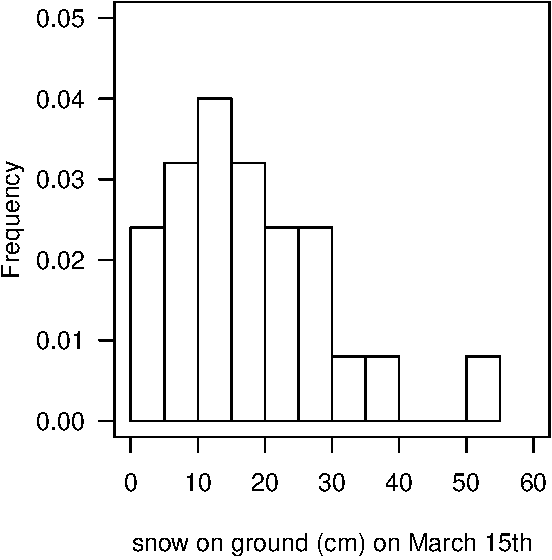
\includegraphics{White_et_al_pika_phenology_supp_mat_files/figure-latex/unnamed-chunk-1-1.pdf}
\caption{Frequency of the amount of snow present (cm) on the ground on
March 15th of each year from 1989-2014. The data is from Environment
Canada Burwash A station (61\degree 22'N, 139\degree 03'W, elevation:
806m).\label{fig:E0_plot}}
\end{figure}

\begin{figure}
\centering
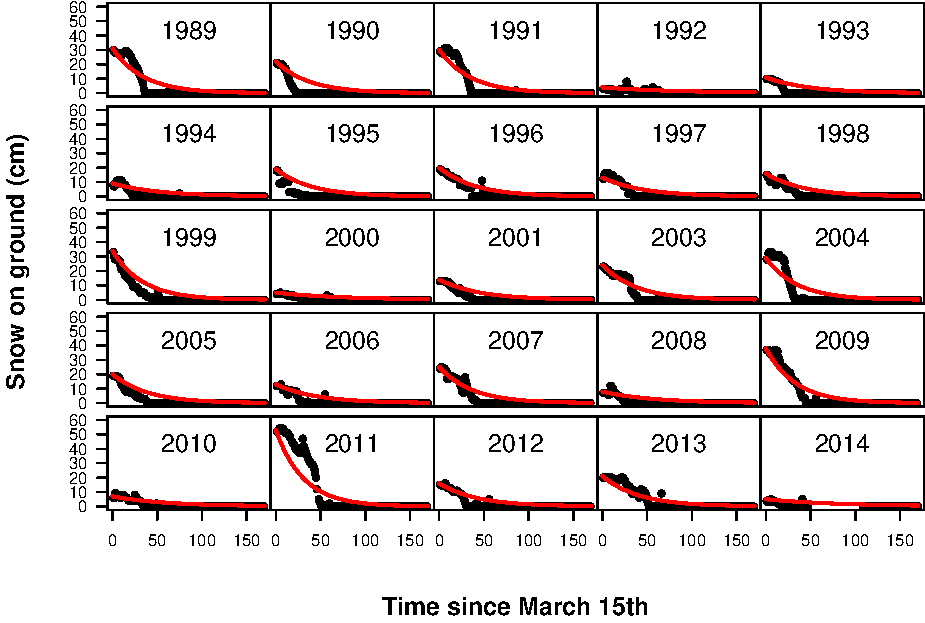
\includegraphics{White_et_al_pika_phenology_supp_mat_files/figure-latex/unnamed-chunk-2-1.pdf}
\caption{Fitted curves for the change in snow depth since March 15th of
each year. The intercept is held constant for each curve
fit.\label{fig:snow_fit_plot}}
\end{figure}

Assuming a constant rate of decay in snow depth, we estimated the decay
parameter, \(\epsilon=\)-0.0234278, using data on daily snow depth over
the past two decades. We estimated a mean snow depth (\(E_0\)) on March
15th to equal 18.48.

\pagebreak

\subsection{Birth rate}

Past work has indicated that pikas in the Yukon have one litter per year
(Franken and Hik 2004) of between 2.1 and 3 individuals (Smith and
Weston 1990). In our model, we assume a birth pulse. Therefore, each
female has all of her offspring within a given year at the same time.
Thus, the number of offspring born in a year is simply the average
number of female offspring (i.e.~we halve the overall birth rate to 1.5)
multiplied by the number of adult females.

\subsection{Adult summer mortality}

There are not field estimates of adult summer mortality, but it is
thought to be low (J.D. Nagy, personal communication). Between
1995-2009, COSEWIC (2011) estimated a yearly mortality rate of 0.63 for
female adult pikas. We assume a modest percentage of mortality occurs in
summer, around 0.15, or a quarter of the yearly mortality rate. We can
use this estimate and solve for \(u_A\) in the within season equation
for adults, we obtain an estimate \(u_A = -0.001\).

\subsection{Juvenile summer mortality}

There are often high rates of mortality for juveniles after birth
(Millar 1974). In addition, pikas are known to abandon entire litters if
weather conditions are poor. Both of these processes act early in the
reproductive season. However, little is known about either process for
our particular species of interest. For a related species,
\emph{Ochotona princeps}, 21\% of offspring may die before weaning
occurs (Millar 1974).

We assume a juvenile summer mortality function that is affected by
current environmental conditions in equation 1 of the main manuscript.
Here, \(u_J\) is the summer mortality rate for juveniles when there is
no snow present, optimal environmental conditions. Then, \(u_E + u_J\)
is the maximum mortality rate when there is a lot of snow present.
Lastly, \(K\) is the half saturation constant, or the amount of snow at
which there is \(u_E/2\) mortality rate, that determines the shape of
the saturating curve between mortality and \(E(t)\).

Unfortunately, there are no published estimates of of these specific
parameters as juveniles are only captured several months after they are
born (Franken and Hik 2004). Weaning mortality occurs between birth and
the time of first capture. Therefore, we used the difference between
number of juveniles captured each year (COSEWIC 2011) and the maximum
birth rate, to try and estimate the juvenile summer (or weaning)
mortality rate. We found that the weaning mortality rate ranged from
0.27 to 0.76 each year.

First, we assumed that juvenile mortality without snow, \(u_J\), was the
same as the adult summer mortality, \(u_A\). Unfortunately, these
parameters were non-identifiable due to the limited number of data
points to estimate such a complicated function. Therefore, we resorted
to using the model itself to estimate \(u_E\) and \(K\). In an average
snowfall year, a value of \(u_E = 0.005\) and \(K = 1\) results in a
summer mortality rate of 28\%, in line with previous work (Millar 1974).

\subsection{Plant consumption}

We assume that plants are consumed by juveniles and adults by Holling
type I or type II functional responses. In the model, we describe
different functions for juveniles and adults, but we assume they have
the same parameter values. In particular, there are two parameters
\(a\), the attack rate. And second, if using a type II response is
\(h\), the handling time.

In our model, \(a\) is the attack rate and is in units area/time as the
amount of resources is given as a density. Biologically, \(a\) is the
amount of area a pika can search during a particular foraging bout.
Pikas only travel short distances during foraging bouts. Unfortunately,
we do not have an estimate of the foraging area covered by pikas during
a single trip. Therefore, we use our model to indirectly estimate
\(a_A\), an inverse modeling procedure (White et al. 2014). In order for
pikas to achieve the mean grams per haypile found by the end of summer
in Morrison et al. (2009), \(a_A\) = 3.

The handling time is the amount of time required for a pika to collect 1
gram of plant material. We do not have a direct estimate of handling
time, but we can use the maximum number of foraging bouts within an hour
to estimate handling time. Each trip takes an estimated 2.4 minutes
(Morrison et al. 2009) and results in on average 0.62 grams of plant
material. This results in a handling time, \(h_A\) of 0.00269 days/gram
food.

In the results of the main text, we focus on a linear (type I)
functional response when the handling time is zero, this simplifies what
attractors are possible.

\subsection{Resource reserve (haypile size)}

Through resource consumption, as described in the previous section, and
the use of those resources, a resource reserve, or haypile size, can
either increase or decrease. We assume resources collected during
foraging are converted into a resource reserve, in this case haypile
size, at a rate determined by \(w_A = 1/3\) (Smith and Ivins 1984). This
rate is calculated as the fraction of time foraging spent haying versus
the combined time spent haying and feeding.

\subsection{Resource decay}

We assume resources, or haypile size, decays at a constant rate. Dearing
(1997) constructed eight artificial haypiles in West Knoll, Colorado.
Dearing (1997) then estimated the amount of biomass loss each month in
summer and winter. We use these results to estimate the decay parameter,
\(\beta\), of haypile size, \(B_A\). We assume this parameter is the
same for both juveniles and adults. In the equation below, 62 is the
number of days over which Dearing (1997) estimated haypile decay at a
study site in Colorado. \[
  B_A(t) = B_A(0) e^{\beta_A t}
  \] \[
  7.3 = 8 e^{\beta_A 62}
  \] \[
  \beta_A = -0.00147 \frac{grams}{day}
  \]

This estimation is probably different at the Yukon site given different
plant material and environmental conditions, but no similar experiments
have been conducted there.

\subsection{Plant growth}

Peak vegetation biomass near talus occurs in late July at the study site
and senescence begins soon thereafter (McIntire and Hik 2005). From past
work, we have estimates of the relative amount of AGB (above ground
biomass) in absence of pikas from pika exclusion plots. McIntire and Hik
(2005) estimated plant abundance is for four different time points
during one summer at the study site. Plant growth increases until July
and then declines before winter begins.

We assume plant growth in the absence of predation is governed by a
simple logistic growth equation. Therefore, both the intrinsic rate of
growth \(r\) and the carrying capacity \(K_R\) need to be estimated. We
use data from the pika-exclusion experiment on plant growth (McIntire
and Hik 2005). Although the data is limited, we were able to fit the
solution to the logistic growth equation to obtain estimates for \(r\)
and \(K_R\) (Fig. \ref{fig:plant_growth}). We assume that growth starts
from a small amount (3 g/\(\mbox{m}^2\)) of biomass each spring.

\begin{figure}
\centering
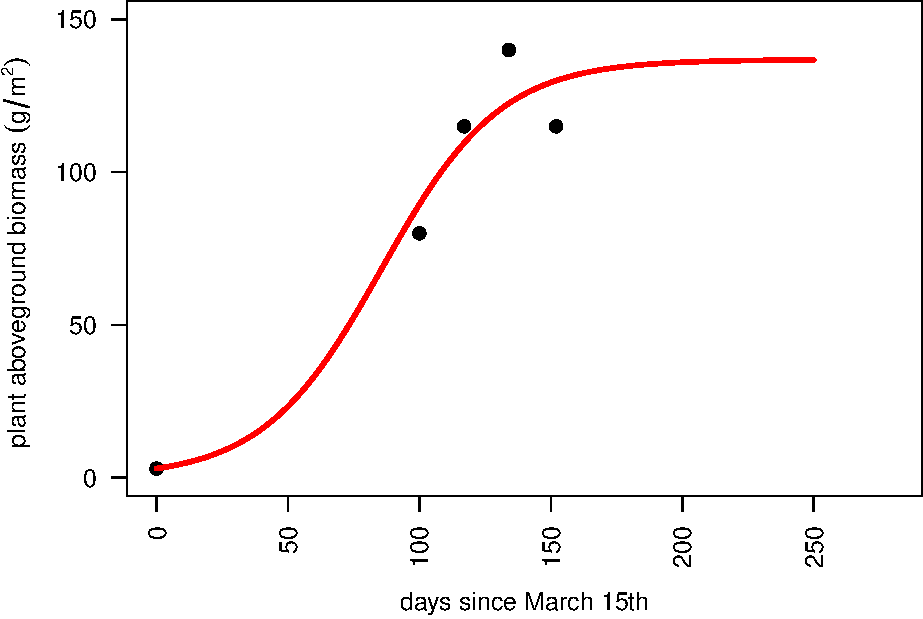
\includegraphics{White_et_al_pika_phenology_supp_mat_files/figure-latex/unnamed-chunk-4-1.pdf}
\caption{Fit of logistic growth model for plant density data found in
McIntire and Hik 2005.\label{fig:plant_growth}}
\end{figure}

Assuming a logistic equation for plant growth, our model estimated
\(r\)=0.0443 and \(K_R\)=136.8244.

\subsection{Over-winter parameterization}

Pikas often experience high over-winter mortality (Morrison and Hik
2007). Their survival depends on the size of their haypile before winter
begins. Therefore, we assumed a saturating function where over-winter
survival depends on haypile size. Morrison et al. (2009) examined
over-winter survival and found it depended on when pikas initiated
haying, and thus their haypile size. We assume a high potential
over-winter survival of 0.9, which is likely rarely achieved as pikas
are not able to build large enough haypiles most years, but it is just a
maximum value. We roughly estimate the half-saturation parameter to be
near \(k_A\) = 2500, based on the probability of survival for pikas over
one winter (Morrison et al. 2009).

We assume that all juvenile pikas either become adults (acquiring a
territory) or die over winter (Smith and Weston 1990). Therefore, we do
not need a function for juvenile over-winter mortality.

\pagebreak

\section{Sensitivity analyses}

Here we illustrate the sensitivity of the predicted evolutionary stable
strategies (ESS) and day of reproductive timing to changes in parameter
values. Assuming no environmental stochasticty, we varied parameters
away from defaults (see Table 1 in main text) and then determined the
ESS and realized reproductive timing. We specifically examined the
juvenile mortality parameters as these were not estimated from field
data. Additionally, we examined the birth rate and over-winter mortality
rate because of their importance in determining evolutionary outcomes.

\begin{figure}
\centering
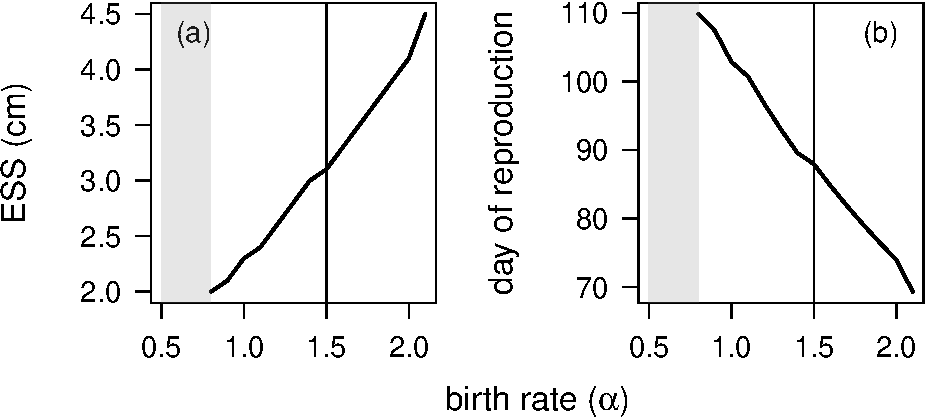
\includegraphics{White_et_al_pika_phenology_supp_mat_files/figure-latex/unnamed-chunk-6-1.pdf}
\caption{(a) Predicted evolutionary stable strategy and (b) day of
reproduction for different values of birth rate (litter size). The light
grey box indicates value of parameter where the population is not
viable. The vertical line is the default parameter value found in Table
1 of the main text. \label{fig:ESS_vs_birth_rate}}
\end{figure}

\begin{figure}
\centering
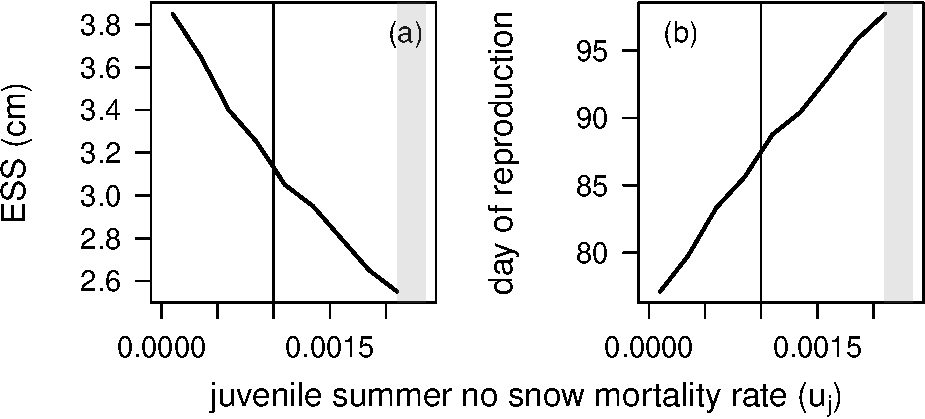
\includegraphics{White_et_al_pika_phenology_supp_mat_files/figure-latex/unnamed-chunk-7-1.pdf}
\caption{(a) Predicted evolutionary stable strategy and (b) day of
reproduction for different values juvenile summer mortality with no snow
present, \(u_J\). The light grey box indicates value of parameter where
the population is not viable. The vertical line is the default parameter
value found in Table 1 of the main text.\label{fig:ESS_vs_u_j}}
\end{figure}

\begin{figure}
\centering
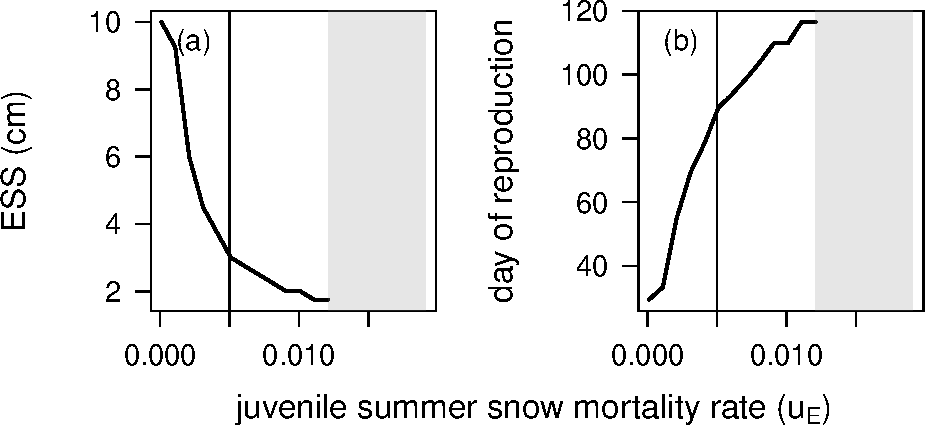
\includegraphics{White_et_al_pika_phenology_supp_mat_files/figure-latex/unnamed-chunk-8-1.pdf}
\caption{(a) Predicted evolutionary stable strategy and (b) day of
reproduction for different values juvenile summer mortality with snow
present, \(u_E\). The light grey box indicates value of parameter where
the population is not viable. The vertical line is the default parameter
value found in Table 1 of the main text.\label{fig:ESS_vs_u_E}}
\end{figure}

\begin{figure}
\centering
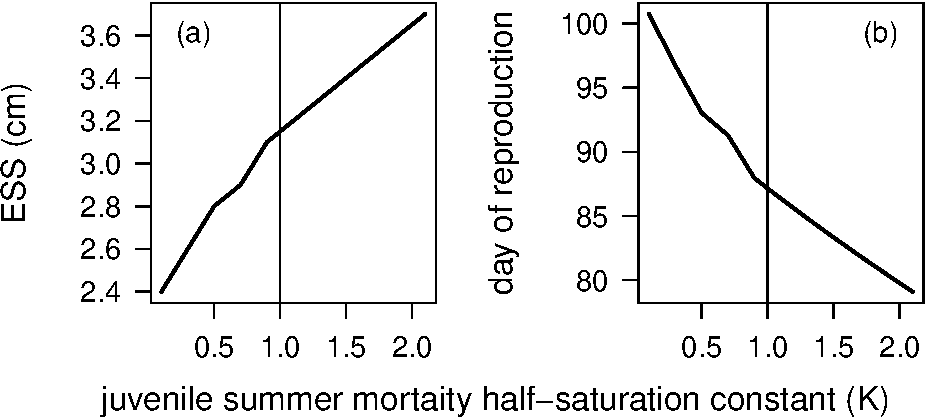
\includegraphics{White_et_al_pika_phenology_supp_mat_files/figure-latex/unnamed-chunk-9-1.pdf}
\caption{(a) Predicted evolutionary stable strategy and (b) day of
reproduction for different values juvenile summer mortality
half-saturation constant, \(K\). A larger value of \(K\) implies pika
mortality increases faster with snow depth. The light grey box indicates
value of parameter where the population is not viable. The vertical line
is the default parameter value found in Table 1 of the main
text.\label{fig:ESS_vs_K}}
\end{figure}

\begin{figure}
\centering
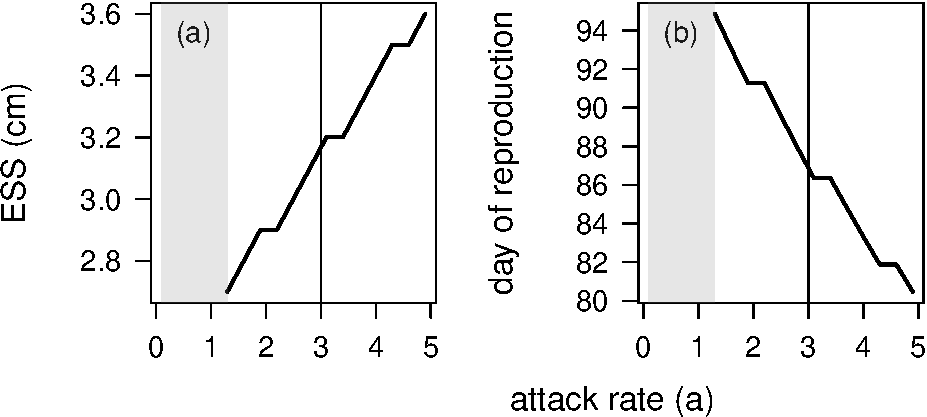
\includegraphics{White_et_al_pika_phenology_supp_mat_files/figure-latex/unnamed-chunk-10-1.pdf}
\caption{(a) Predicted evolutionary stable strategy and (b) day of
reproduction for different values of attack rate for both juveniles
(\(a_J\)) and adults (\(a_A\)). The light grey box indicates value of
parameter where the population is not viable. The vertical line is the
default parameter value found in Table 1 of the main
text.\label{fig:ESS_vs_attack_rate}}
\end{figure}

\begin{figure}
\centering
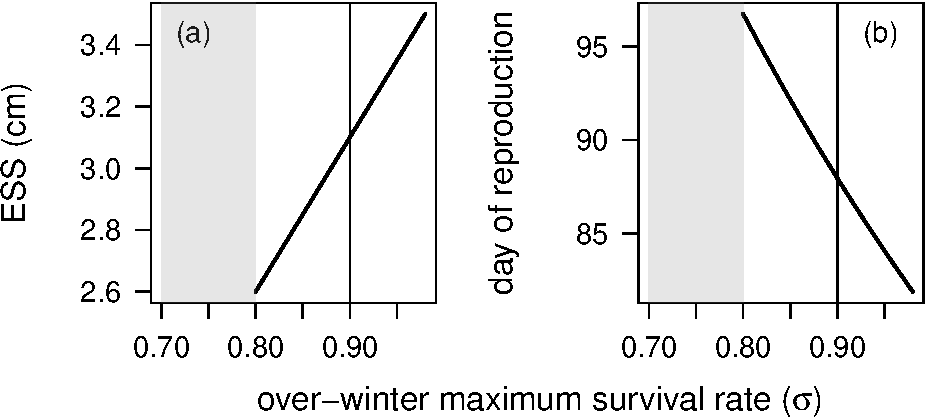
\includegraphics{White_et_al_pika_phenology_supp_mat_files/figure-latex/unnamed-chunk-11-1.pdf}
\caption{(a) Predicted evolutionary stable strategy and (b) day of
reproduction for different values of maximum over-winter survival rate
for both juveniles (\(\sigma_J\)) and adults (\(\sigma_A\)). The light
grey box indicates value of parameter where the population is not
viable. The vertical line is the default parameter value found in Table
1 of the main text.\label{fig:ESS_vs_over_winter}}
\end{figure}

\pagebreak

\section{References}\label{references}

\hypertarget{refs}{}
\hypertarget{ref-COSEWIC2011}{}
COSEWIC. 2011. COSEWIC assessment and status report on the Collared Pika
(Ochotona collaris) in Canada. Page 50. Committee on the Status of
Endangered Wildlife in Canada, Ottawa.

\hypertarget{ref-Dearing1997}{}
Dearing, M. D. 1997. The function of haypiles of pikas. Journal of
Mammalogy 78:1156--1163.

\hypertarget{ref-Franken2004b}{}
Franken, R. J., and D. S. Hik. 2004. Interannual variation in timing of
parturition and growth of collared pikas (Ochotona collaris) in the
Southwest Yukon. Integrative and Comparative Biology 44:186--93.

\hypertarget{ref-McIntire2005}{}
McIntire, E. J. B., and D. S. Hik. 2005. Influences of chronic and
current season grazing by collared pikas on above-ground biomass and
species richness in subarctic alpine meadows. Oecologia 145:288--297.

\hypertarget{ref-Millar1974}{}
Millar, J. C. 1974. Success of reproduction in pikas, Ochotona princeps.
Journal of Mammalogy 55:527--542.

\hypertarget{ref-Morrison2007}{}
Morrison, S. F., and D. S. Hik. 2007. Demographic analysis of a
declining pika Ochotona collaris population: Linking survival to
broad-scale climate patterns via spring snowmelt patterns. Journal of
Animal Ecology 76:899--907.

\hypertarget{ref-Morrison2009}{}
Morrison, S. F., G. Pelchat, A. Donahue, and D. S. Hik. 2009. Influence
of food hoarding behavior on the over-winter survival of pikas in
strongly seasonal envrionments. Oecologia 157:107--116.

\hypertarget{ref-Smith1984a}{}
Smith, A. T., and B. L. Ivins. 1984. Spatial relationships and social
organization in adult pikas - a facultatively monogaous mammal.
Zeitschrift fur Tierpsychologie 66:289--308.

\hypertarget{ref-SmithWeston1990}{}
Smith, A. T., and M. L. Weston. 1990. Ochotona princeps. Mammalian
Species 352:392--397.

\hypertarget{ref-White2014}{}
White, E. R., J. D. Nagy, and S. H. Gruber. 2014. Modeling the
population dynamics of lemon sharks. Biology Direct 9:1--18.


\end{document}
